\section{Results}

A summary of the background expectations and the corresponding data counts for each signal
region is shown in Table \ref{tab:results} and shown in Fig/\ref{fig:results}.  The observed and predicted yields agree in all signal regions within about XX standard deviations. Therefore, we observe no evidence for top-squark pair production.

\begin{table}[htb]
\begin{center}
\caption{\label{tab:results} Results of the data- and simulation-driven background estimates together with the observed data yields for 2.3\fbinv collected during 2015 pp collisions. The uncertainties are the quadratic sums of statistical and systematic uncertainties.{\color{red} Data still blinded.}}
\begin{tabular}{|r|r@{\,$\pm$\,}lr@{\,$\pm$\,}lr@{\,$\pm$\,}lr@{\,$\pm$\,}l|r@{\,$\pm$\,}l|r|}
\hline
\multirow{2}{*}{\MET [GeV]} &  \multicolumn{2}{c|}{\multirow{2}{*}{Lost Lepton}} & \multicolumn{2}{c|}{$1\ell$ (not}  &  \multicolumn{2}{c|}{\multirow{2}{*}{$\ttbar\to1\ell$}} &  \multicolumn{2}{c|}{\multirow{2}{*}{$\cPZ\to\cPgn\cPagn$}} & \multicolumn{2}{c|}{Total} & \multirow{2}{*}{Data} \\
 & \multicolumn{2}{c|}{~} & \multicolumn{2}{c|}{from top)} & \multicolumn{2}{c|}{~} & \multicolumn{2}{c|}{~} & \multicolumn{2}{c|}{background} &  \\
\hline
 & \multicolumn{11}{l|}{Boosted High $\Delta M$}\\%: $3$ jets, $\MTtW>200\GeV$} \\
\hline
$>350$    & 0.84&0.23 & 0.98&0.62 & 0.05&0.05 & 0.28&0.08 & 2.15&0.67 & 0 \\
\hline
 & \multicolumn{11}{l|}{Low $\Delta M$}\\%: $\geq4$ jets, $\MTtW\leq200\GeV$} \\
\hline
$250-325$ & 19.27&2.76 & 0.55&0.55 & 0.76&0.76 & 0.63&0.12 & 21.21&2.92 & 0 \\
$>325$ & 7.64&1.28 & 0.38&0.38 & 0.34&0.34 & 0.27&0.08 & 8.63&1.38 & 0 \\
\hline
 & \multicolumn{11}{l|}{High $\Delta M$}\\%: $\geq4$ jets, $\MTtW>200\GeV$} \\
\hline
$250-350$ & 3.08&0.82 & 1.05&0.53 & 0.49&0.49 & 0.63&0.15 & 5.25&1.10 & 0 \\
$350-450$ & 0.83&0.23 & 0.82&0.49 & 0.12&0.12 & 0.38&0.10 & 2.15&0.56 & 0 \\
$>450$ & 0.59&0.21 & 0.95&0.67 & 0.07&0.07 & 0.34&0.15 & 1.95&0.72 & 0 \\
\hline
\end{tabular}
\end{center}
\end{table}

\begin{figure}[htb]
\centering
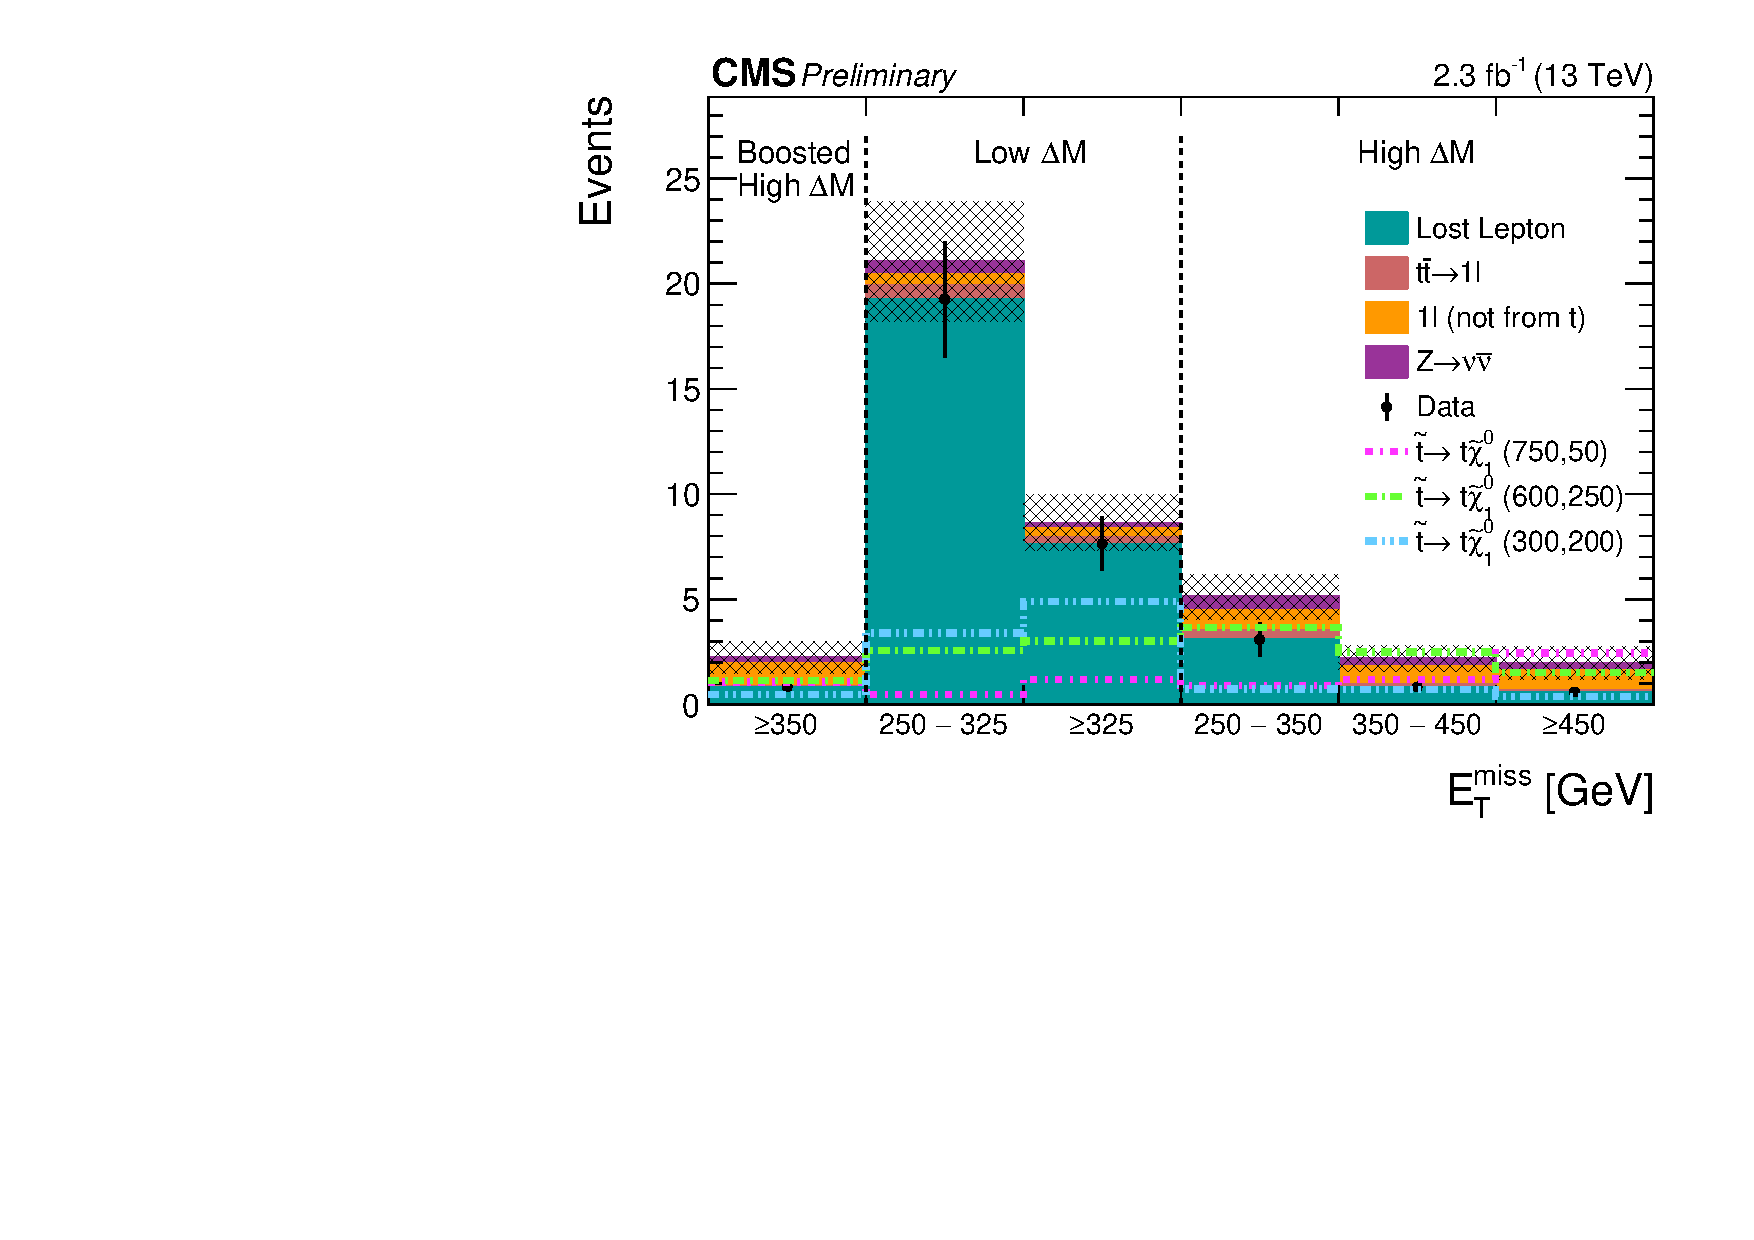
\includegraphics[width=0.90\textwidth]{plots_stop/Results_2p3fbinv.pdf}
\caption{\label{fig:results}Results of the data- and simulation-driven background estimates together with the observed data yields for 2.3\fbinv collected during 2015 pp collisions. The uncertainties, which are the quadratic sums of statistical and systematic uncertainties, are shown as shaded band. Three signal hypotheses are overlaid. {\color{red} Data still blinded, dots here are fake.}}
\end{figure}

The results of the search are interpreted in the context of models of top-squark pair production.  As discussed in Sec.\ref{sec:intro} we consider two different decay modes for the top-squark: directly to a top quark and a LSP or to a bottom quark and a chargino and then the chargino decays to the LSP.  We also consider the option where the chargino is almost mass-degenerate with the LSP.  In that case we can be sensitive to the mixed scenario, where one top decays to a top quark and a LSP and the other one to a bottom quark, a soft and undetected W boson and a LSP.  The systematic uncertainties are discussed in length in Sec.\ref{syst}.  We use all the search bins to calculate 95\% confidence level (CL) upper limits (UL) on the cross sections.  We calculate these upper limits using the LHC style CL$_{S}$ method\cite{Higgscombine}.

Figure~\ref{fig:limits:T2tt} shows the 95\% CL exclusion limits for $\Pp\Pp\to\stone\stone^*\to \PQt^{(*)}\PAQt^{(*)}\PSGczDo\PSGczDo$, together with the upper limit at 95\% CL on the excluded signal cross section.
\begin{figure}[htb]
\centering
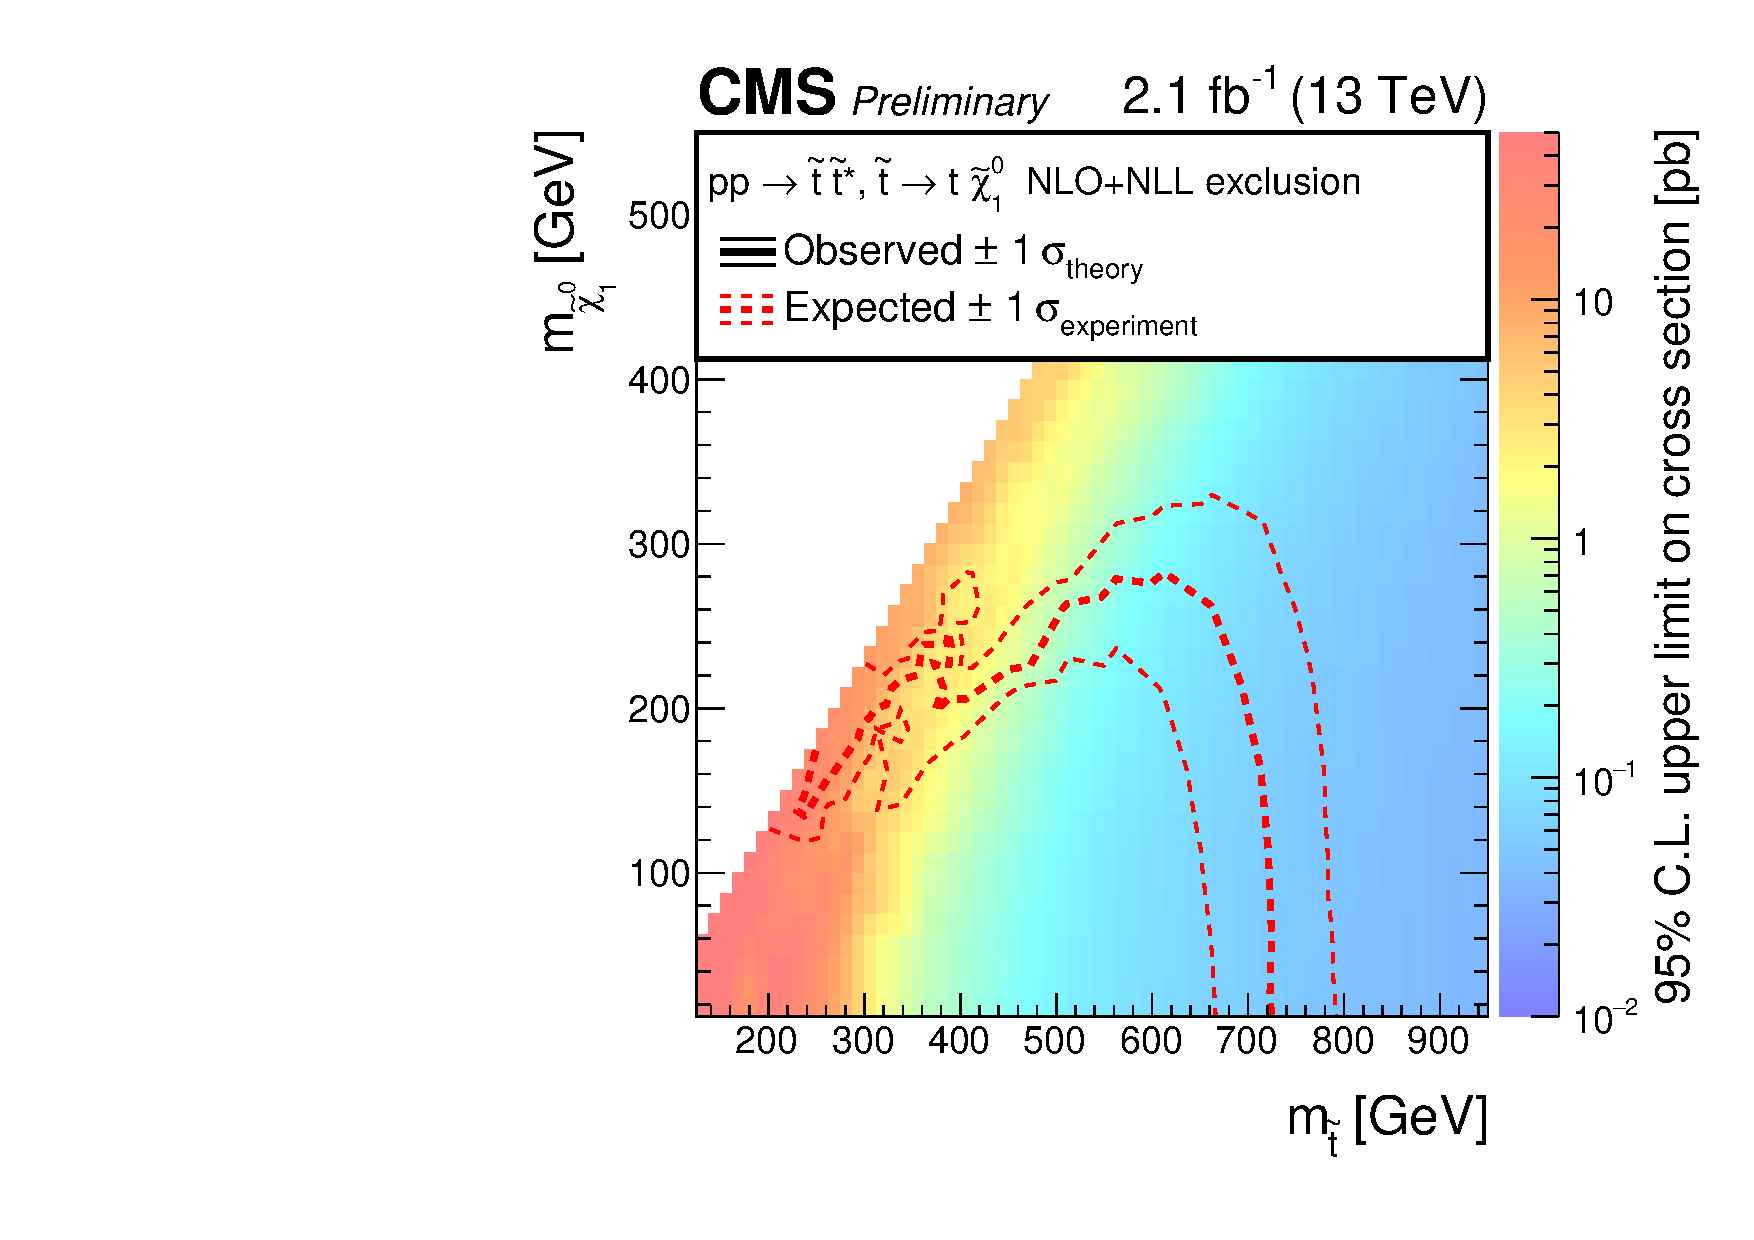
\includegraphics[width=0.8\textwidth]{plots_stop/T2ttstopXSEC.pdf}
\caption{\label{fig:limits:T2tt}Exclusion limit at 95\% CL for direct top-squark production with decay $\stone\to\PQt^{(*)}\PSGczDo$. \textcolor{red}{Once the final plot is here, we also need to add information about the different lines...} }
\end{figure}

\textcolor{red}{Section not finished yet.}
